\documentclass[12pt]{article}
\usepackage{xeCJK}
\usepackage{tikz}
\usetikzlibrary{calc}
\usetikzlibrary{shapes.geometric}
\usetikzlibrary{positioning}
\usetikzlibrary {arrows.meta}
\setCJKmainfont{NotoSerifTC-Regular.otf}
\title{Tikz Figures}
\author{Cheng, Jui-Hung}

\begin{document}
\maketitle

\begin{figure}
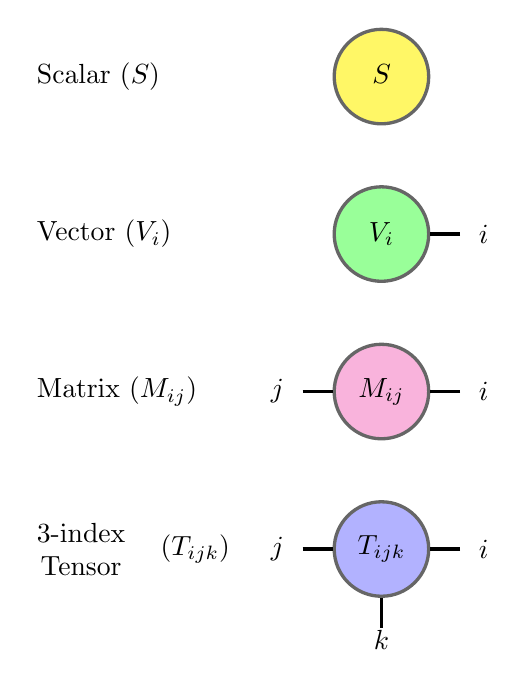
\begin{tikzpicture}[
    roundnode/.style={circle, draw=black!60, very thick, minimum size=12mm},
]
    % Scalar
    \node (scalar_title) at (0, 7)[right=-2cm]{Scalar ($ S_{} $)};
    \node at (2.5, 7) [roundnode, fill=yellow!60](scalar){$S_{}$};
    
    % Vector
    \node (vector_title) at (0, 5)[right=-2cm]{Vector ($ V_{i} $)};
    \node at (2.5, 5) [roundnode, fill=green!40](vector){$V_i$};
    \draw [very thick] (3.5, 5) -- (vector.east) (3.5, 5) node[right= 0.1cm]{$i$} ;

    % Matrix
    \node (matrix_title) at (0, 3)[right=-2cm]{Matrix ($ M_{ij} $)};
    \node at (2.5, 3) [roundnode, fill=magenta!30](matrix){$M_{ij}$};
    \draw [very thick] (3.5, 3) -- (matrix.east) (3.5, 3) node[right= 0.1cm]{$i$} ;
    \draw [very thick] (1.5, 3) -- (matrix.west) (1.5, 3) node[left= 0.1cm]{$j$} ;

    % Tensor
    \node (tensor_title) at (0, 1)[right=-2cm, align=center]{3-index \\ Tensor};
    \node at (0.7, 1) [anchor=east] {($T_{ijk}$)}; 
    \node at (2.5, 1) [roundnode, fill=blue!30](tensor){$T_{ijk}$};
    \draw [very thick] (3.5, 1) -- (tensor.east) (3.5, 1) node[right= 0.1cm]{$i$} ;
    \draw [very thick] (1.5, 1) -- (tensor.west) (1.5, 1) node[left= 0.1cm]{$j$} ;
    \draw [very thick] (2.5, 0) -- (tensor.south) (2.5, 0.2) node[below= 0.1cm]{$k$} ;
    
\end{tikzpicture}
\caption{Tensor Diagrams} \label{fig:Tensor Diagrams}
\end{figure}

\begin{figure}
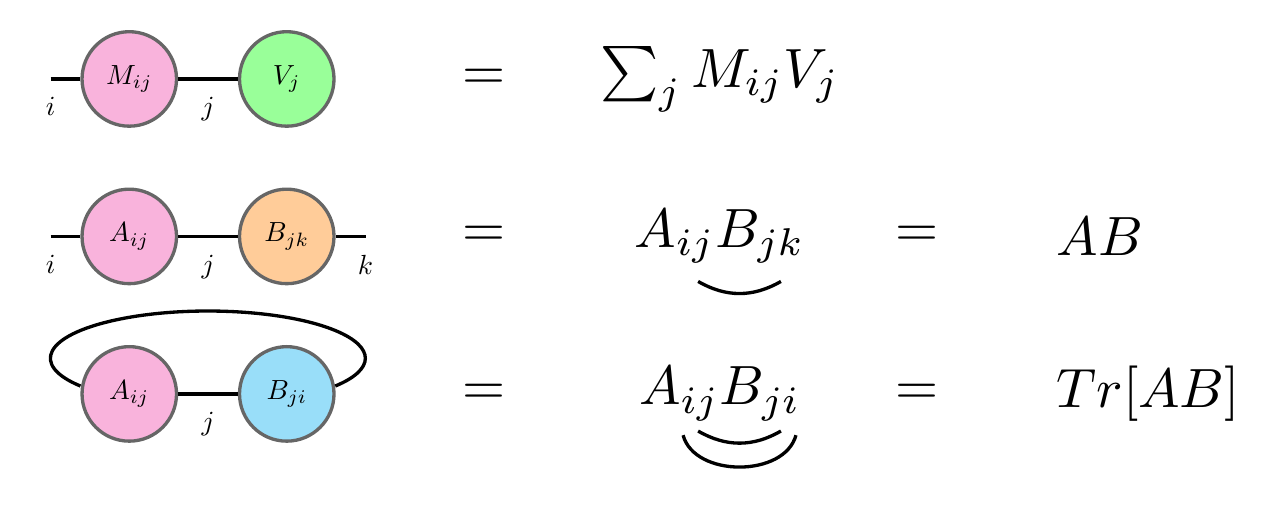
\begin{tikzpicture}[
    roundnode/.style={circle, draw=black!60, very thick, minimum size=12mm}
]
    % Matrix add Vector
    % - [Fig: Matrix add Vector]
    \node at (2.5, 5) [roundnode, fill=magenta!30](matrix){$M_{ij}$};
    \node at (4.5, 5) [roundnode, fill=green!40](vector){$V_{j}$};
    % -- The i branch of matrix
    \draw [very thick] (1.5, 5) -- (matrix.west) (1.5, 5) node[below= 0.1cm]{$i$} ;
    % -- Calculate the midpoint
    \coordinate (midpoint) at ($(matrix.east)!0.5!(vector.west)$);
    \draw [very thick] (matrix.east) -- (vector.west) (midpoint) node[below= 0.1cm]{$j$} ;
    % - [Formula Explanation]
    \node at (7, 5) [scale=2, very thick, ]{=} ;
    \node at (10, 5) [scale=2, very thick, ]{$\sum_{j}^{}{M_{ij}V_{j}} $} ;

   
    % Matrix add Matrix
    % - [Fig: Matrix add Matrix]
    \node at (2.5, 3) [roundnode, fill=magenta!30](matrix_A){$A_{ij}$};
    \node at (4.5, 3) [roundnode, fill=orange!40](matrix_B){$B_{jk}$};
    % -- The branch i of matrix_A
    \draw [very thick] (1.5, 3) -- (matrix_A.west) (1.5, 3) node[below= 0.1cm]{$i$} ;
    % -- The branch k of matrix_B
    \draw [very thick] (5.5, 3) -- (matrix_B.east) (5.5, 3) node[below= 0.1cm]{$k$} ;
    % -- Connect the matrix_A and matrix_B
    % --- Calculate the midpoint of A B
    \coordinate (midpoint) at ($(matrix_A.east)!0.5!(matrix_B.west)$);
    \draw [very thick] (matrix_A.east) -- (matrix_B.west) (midpoint) node[below= 0.1cm]{$j$} ;
    % - [Formula Explanation]
    \node at (7, 3) [scale=2, very thick, ]{=} ;
    \node at (10, 3) [scale=2, very thick, ]{$ {A_{ij}B_{jk}} $} ;
    \node at (9.6, 2.5) [] (j_1) {} ;
    \node at (10.9, 2.5) [] (j_2) {} ;
    \path [very thick, bend right] (j_1) edge (j_2) ;
    % - [Formula Result]
    \node at (12.5, 3) [scale=2, very thick, ]{=} ;
    \node at (15, 3) [scale=2, very thick, right=-1cm]{$AB$} ;


    % Matrix add Matrix connect head and tail
    % - [Fig: Matrix add Matrix]
    \node at (2.5, 1) [roundnode, fill=magenta!30](matrix_A){$A_{ij}$};
    \node at (4.5, 1) [roundnode, fill=cyan!40](matrix_B){$B_{ji}$};
    % -- Connect the matrix_A and matrix_B 
    % --- Calculate the midpoint of A B 
    \coordinate (midpoint) at ($(matrix_A.east)!0.5!(matrix_B.west)$);
    \draw [very thick] (matrix_A.east) -- (matrix_B.west) (midpoint) node[below= 0.1cm]{$j$} ;
    % -- Arc on the Figures
    \draw (midpoint) [very thick] ([xshift=-1.62cm, yshift=0.1cm] midpoint) arc (216:-36:2cm and 0.6cm);
    % - [Formula Explanation]
    \node at (7, 1) [scale=2, very thick, ]{=} ;
    \node at (10, 1) [scale=2, very thick, ]{${A_{ij}B_{ji}} $} ;
    % -- the curve of j and i
    \node at (9.6, 0.6) [] (j_1) {} ;
    \node at (10.9, 0.6) [] (j_2) {} ;
    \path [very thick, bend right] (j_1) edge (j_2) ;
    \node at (9.5, 0.6) [] (i_1) {} ;
    \node at (11.0, 0.6) [] (i_2) {} ;
    \path [very thick, bend right, out=-75, in=-105] (i_1) edge (i_2) ;
    % - [Formula Result]
    \node at (12.5, 1) [scale=2, very thick, ]{=} ;
    \node at (15, 1) [scale=2, very thick, right=-1cm]{$Tr[AB]$} ;
    
\end{tikzpicture}
\caption{Sample Contractions} \label{fig:Sample Contractions}
\end{figure}

\begin{figure}
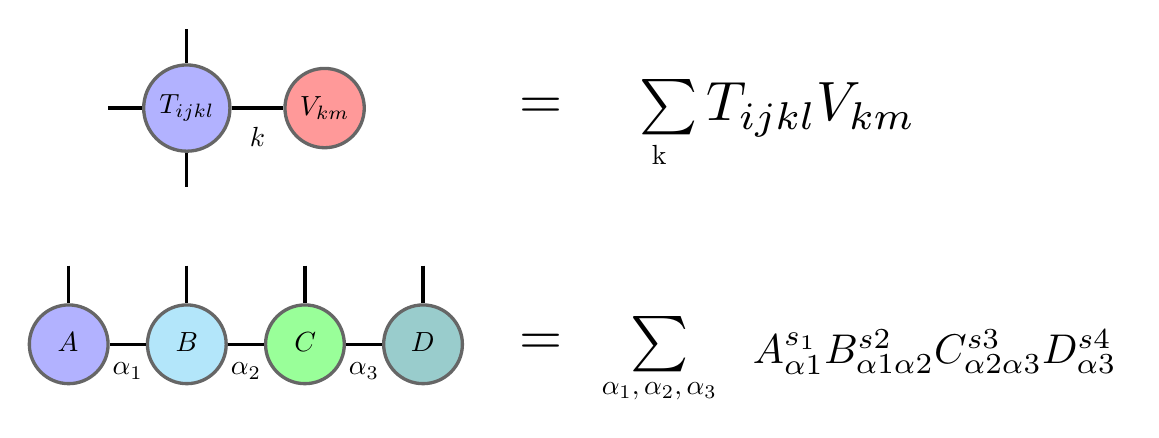
\begin{tikzpicture}[
    roundnode/.style={circle, draw=black!60, very thick, minimum size=10mm}
]
    % Tensor add Matrix
    % - [Fig: Tensor add Matrix]
    \node at (2.5, 5) [roundnode, fill=blue!30](matrix){$T_{ijkl}$};
    \node at (4.25, 5) [roundnode, fill=red!40](vector){$V_{km}$};
    % -- The branches of tensor
    \draw [very thick] (1.5, 5) -- (matrix.west) ;
    \draw [very thick] (2.5, 6) -- (matrix.north) ;
    \draw [very thick] (2.5, 4) -- (matrix.south) ;
    
    % -- Calculate the midpoint
    \coordinate (midpoint) at ($(matrix.east)!0.5!(vector.west)$);
    \draw [very thick] (matrix.east) -- (vector.west) (midpoint) node[below= 0.1cm]{$k$} ;
    % - [Formula Explanation]
    \node at (7, 5) [scale=2, very thick, ]{=} ;
    % comment: should the vector V change to matrix M, since it is a 2-dimension matrix
    \node at (10, 5) [scale=2, very thick, ]{$\sum{T_{ijkl}V_{km}} $} ;
    \node at (8.5, 4.4) [scale = 1, very thick, ]{k} ;
    
    % Matrix add Matrix
    % - [Fig: Matrix add Matrix]
    \node at (1, 2) [roundnode, fill=blue!30](matrix_A){$A_{}$};
    \node at (2.5, 2) [roundnode, fill=cyan!30](matrix_B){$B_{}$};
    \node at (4, 2) [roundnode, fill=green!40](matrix_C){$C_{}$};
    \node at (5.5, 2) [roundnode, fill=teal!40](matrix_D){$D_{}$};
    % -- Connect the matrix left and matrix right
    % --- Calculate the midpoint
    \coordinate (midAB) at ($(matrix_A.east)!0.5!(matrix_B.west)$);
    \draw [very thick] (matrix_A.east) -- (matrix_B.west) (midAB) node[below= 0.1cm]{$\alpha_1$} ;
    \coordinate (midBC) at ($(matrix_B.east)!0.5!(matrix_C.west)$);
    \draw [very thick] (matrix_B.east) -- (matrix_C.west) (midBC) node[below= 0.1cm]{$\alpha_2$} ;
    \coordinate (midCD) at ($(matrix_C.east)!0.5!(matrix_D.west)$);
    \draw [very thick] (matrix_C.east) -- (matrix_D.west) (midCD) node[below= 0.1cm]{$\alpha_3$} ;
    % -- The branches of matrices
    \draw [very thick] (1, 3) -- (matrix_A.north) ;
    \draw [very thick] (2.5, 3) -- (matrix_B.north) ;
    \draw [very thick] (4, 3) -- (matrix_C.north) ;
    \draw [very thick] (5.5, 3) -- (matrix_D.north) ;
    % - [Formula Explanation]
    \node at (7, 2) [scale=2, very thick, ]{=} ;
    \node at (8.5, 2) [scale=2, very thick, ]{$\sum$${} $} ;
    \node at (8.5, 1.4) [scale = 1, very thick, ]{$\alpha_1, \alpha_2, \alpha_3$} ;
    \node at (12, 1.9) [scale=1.5, very thick, ]{${A^{s_1}_{\alpha1} B^{s2}_{\alpha1\alpha2}} C^{s3}_{\alpha2\alpha3}  D^{s4}_{\alpha3} $} ;
    

\end{tikzpicture}
\caption{Tensor Contractions} \label{fig:Tensor Contractions}
\end{figure}


\begin{figure}
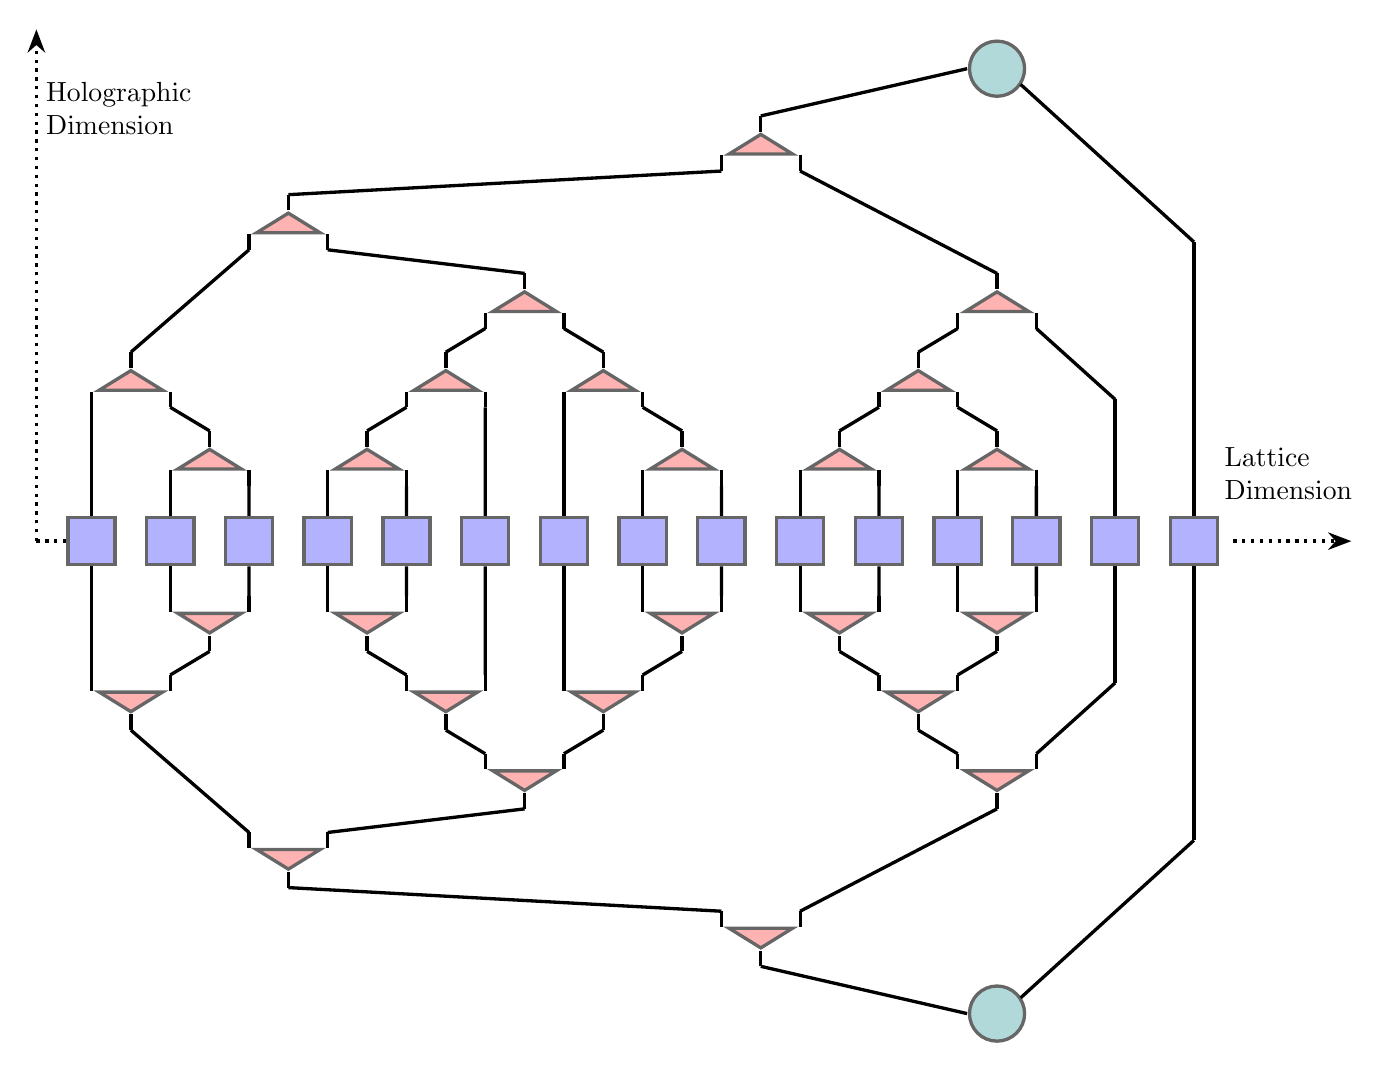
\begin{tikzpicture}[
    scale=1,
    rectnode/.style={rectangle, draw=black!60, very thick, minimum size=6mm}, 
    triangle/.style = {fill=red!30, draw=black!60, very thick, regular polygon, regular polygon sides=3, yscale=0.5, xscale=1.4 },
    roundnode/.style={circle, fill=teal!30, draw=black!60, very thick, minimum size=7mm},
    border_rotated/.style = {shape border rotate=180},
]

    % the squares
    \foreach \x [count=\i] in {1, ..., 15}
    {
        \node at (\x, 5) [rectnode, fill=blue!30](square){};
        \coordinate (square_upper_\i) at (\x, 5.32) ;
        \coordinate (square_bottom_\i) at (\x, 4.68) ;
    }
    
    % extend the square 14 and 15 which does not connect by the lower triangle
    \foreach \x in {14, 15}
    {
        \coordinate (extend_square_upper_\x) at ($(\x, 6.8) + 2*(0, \x-14)$) ;
        \coordinate (extend_square_bottom_\x) at ($(\x, 3.2) - 2*(0, \x-14) $) ;
        \draw [very thick] (square_upper_\x) -- (extend_square_upper_\x) ;
        \draw [very thick] (square_bottom_\x) -- (extend_square_bottom_\x) ;
    }

    % the labels of Holographic Dimensions
    \draw [very thick, dotted] (0.3, 5) -- (0.7, 5) ;
    \draw [-Stealth] [very thick, dotted] (0.3, 5) -- (0.3, 11.5) ;
    \node at (0.3, 10.5) [align=left, anchor=west](){Holographic \\ Dimension};
    % the labels of Lattice Dimension
    \draw [-Stealth] [very thick, dotted] (15.5, 5) -- (17, 5) ;
    \node at (16.2, 5.4) [align=left, anchor=south](){Lattice \\ Dimension};
    

    % the level 1 triangles
    \foreach \x [count=\i] in {2, 4, 8, 10, 12}
    {
        % the upper triangle
        \node at (\x+0.5, 6) [triangle](triangle){};
        % - the legs of triangle
        \coordinate (left_leg_upper_1_\i) at ($(triangle)+(-0.5, -0.3)$) ;
        \coordinate (right_leg_upper_1_\i) at ($(triangle)+(+0.5, -0.3)$) ;
        \draw [very thick] (left_leg_upper_1_\i) -- ($(left_leg_upper_1_\i)+(0, 0.2)$) ;
        \draw [very thick] (right_leg_upper_1_\i) -- ($(right_leg_upper_1_\i)+(0, 0.2)$) ;
        % - the head of triangle 
        \coordinate (head_upper_1_\i) at ($(triangle)+(0, +0.4)$) ;
        \draw [very thick] (head_upper_1_\i) -- ($(head_upper_1_\i)-(0, 0.2)$) ;
        
        % the bottom triangle
        \node at (\x+0.5, 4) [triangle, border_rotated ,fill=red!30](triangle){};
        % - two legs of triangles
        \coordinate (left_leg_bottom_1_\i) at ($(triangle)+(-0.5, +0.3)$) ;
        \coordinate (right_leg_bottom_1_\i) at ($(triangle)+(+0.5, +0.3)$) ;
        \draw [very thick] (left_leg_bottom_1_\i) -- ($(left_leg_bottom_1_\i)-(0, 0.2)$) ;
        \draw [very thick] (right_leg_bottom_1_\i) -- ($(right_leg_bottom_1_\i)-(0, 0.2)$) ;
        % - the head of triangle
        \coordinate (head_bottom_1_\i) at ($(triangle)+(0, -0.4)$) ;
        \draw [very thick] (head_bottom_1_\i) -- ($(head_bottom_1_\i)+(0, 0.2)$) ;
        
    }
    
    % the level 2 triangles
    \foreach \x [count=\i] in {1.5, 5.5, 7.5, 11.5}
    {
        % the upper triangle
        \node at (\x, 7) [triangle](triangle){};
        % - the legs of triangle
        \coordinate (left_leg_upper_2_\i) at ($(triangle)+(-0.5, -0.3)$) ;
        \coordinate (right_leg_upper_2_\i) at ($(triangle)+(+0.5, -0.3)$) ;
        \draw [very thick] (left_leg_upper_2_\i) -- ($(left_leg_upper_2_\i)+(0, 0.2)$) ;
        \draw [very thick] (right_leg_upper_2_\i) -- ($(right_leg_upper_2_\i)+(0, 0.2)$) ;
        % - the head of triangle
        \coordinate (head_upper_2_\i) at ($(triangle)+(0, +0.4)$) ;
        \draw [very thick] (head_upper_2_\i) -- ($(head_upper_2_\i)-(0, 0.2)$) ;
        
        % the bottom triangle
        \node at (\x, 3) [triangle, border_rotated ,fill=red!30](triangle){};
        % - two legs of triangles
        \coordinate (left_leg_bottom_2_\i) at ($(triangle)+(-0.5, +0.3)$) ;
        \coordinate (right_leg_bottom_2_\i) at ($(triangle)+(+0.5, +0.3)$) ;
        \draw [very thick] (left_leg_bottom_2_\i) -- ($(left_leg_bottom_2_\i)-(0, 0.2)$) ;
        \draw [very thick] (right_leg_bottom_2_\i) -- ($(right_leg_bottom_2_\i)-(0, 0.2)$) ;
        % - the head of triangle
        \coordinate (head_bottom_2_\i) at ($(triangle)+(0, -0.4)$) ;
        \draw [very thick] (head_bottom_2_\i) -- ($(head_bottom_2_\i)+(0, 0.2)$) ;
        
    }

    % the level 3 triangles
    \foreach \x [count=\i] in {6.5, 12.5}
    {
        % the upper triangle
        \node at (\x, 8) [triangle](triangle){};
        % - the legs of triangle
        \coordinate (left_leg_upper_3_\i) at ($(triangle)+(-0.5, -0.3)$) ;
        \coordinate (right_leg_upper_3_\i) at ($(triangle)+(+0.5, -0.3)$) ;
        \draw [very thick] (left_leg_upper_3_\i) -- ($(left_leg_upper_3_\i)+(0, 0.2)$) ;
        \draw [very thick] (right_leg_upper_3_\i) -- ($(right_leg_upper_3_\i)+(0, 0.2)$) ;
        % - the head of triangle
        \coordinate (head_upper_3_\i) at ($(triangle)+(0, +0.4)$) ;
        \draw [very thick] (head_upper_3_\i) -- ($(head_upper_3_\i)-(0, 0.2)$) ;
        
        % the bottom triangle
        \node at (\x, 2) [triangle, border_rotated ,fill=red!30](triangle){};
        % - two legs of triangles
        \coordinate (left_leg_bottom_3_\i) at ($(triangle)+(-0.5, +0.3)$) ;
        \coordinate (right_leg_bottom_3_\i) at ($(triangle)+(+0.5, +0.3)$) ;
        \draw [very thick] (left_leg_bottom_3_\i) -- ($(left_leg_bottom_3_\i)-(0, 0.2)$) ;
        \draw [very thick] (right_leg_bottom_3_\i) -- ($(right_leg_bottom_3_\i)-(0, 0.2)$) ;
        % - the head of triangle
        \coordinate (head_bottom_3_\i) at ($(triangle)+(0, -0.4)$) ;
        \draw [very thick] (head_bottom_3_\i) -- ($(head_bottom_3_\i)+(0, 0.2)$) ;
    
    }

    % the level 4 triangles
    \foreach \x [count=\i] in {3.5}
    {
        % the upper triangle
        \node at (\x, 9) [triangle](triangle){};
        % - the legs of triangle
        \coordinate (left_leg_upper_4_\i) at ($(triangle)+(-0.5, -0.3)$) ;
        \coordinate (right_leg_upper_4_\i) at ($(triangle)+(+0.5, -0.3)$) ;
        \draw [very thick] (left_leg_upper_4_\i) -- ($(left_leg_upper_4_\i)+(0, 0.2)$) ;
        \draw [very thick] (right_leg_upper_4_\i) -- ($(right_leg_upper_4_\i)+(0, 0.2)$) ;
        % - the head of triangle
        \coordinate (head_upper_4_\i) at ($(triangle)+(0, +0.4)$) ;
        \draw [very thick] (head_upper_4_\i) -- ($(head_upper_4_\i)-(0, 0.2)$) ;
        
        % the bottom triangle
        \node at (\x, 1) [triangle, border_rotated ,fill=red!30](triangle){};
        % - two legs of triangles
        \coordinate (left_leg_bottom_4_\i) at ($(triangle)+(-0.5, +0.3)$) ;
        \coordinate (right_leg_bottom_4_\i) at ($(triangle)+(+0.5, +0.3)$) ;
        \draw [very thick] (left_leg_bottom_4_\i) -- ($(left_leg_bottom_4_\i)-(0, 0.2)$) ;
        \draw [very thick] (right_leg_bottom_4_\i) -- ($(right_leg_bottom_4_\i)-(0, 0.2)$) ;
        % - the head of triangle
        \coordinate (head_bottom_4_\i) at ($(triangle)+(0, -0.4)$) ;
        \draw [very thick] (head_bottom_4_\i) -- ($(head_bottom_4_\i)+(0, 0.2)$) ;

    }

    % the level 5 triangles
    \foreach \x [count=\i] in {9.5}
    {
        % the upper triangle
        \node at (\x, 10) [triangle](triangle){};
        % - the legs of triangle
        \coordinate (left_leg_upper_5_\i) at ($(triangle)+(-0.5, -0.3)$) ;
        \coordinate (right_leg_upper_5_\i) at ($(triangle)+(+0.5, -0.3)$) ;
        \draw [very thick] (left_leg_upper_5_\i) -- ($(left_leg_upper_5_\i)+(0, 0.2)$) ;
        \draw [very thick] (right_leg_upper_5_\i) -- ($(right_leg_upper_5_\i)+(0, 0.2)$) ;
        % - the head of triangle
        \coordinate (head_upper_5_\i) at ($(triangle)+(0, +0.4)$) ;
        \draw [very thick] (head_upper_5_\i) -- ($(head_upper_5_\i)-(0, 0.2)$) ;
        
        % the bottom triangle
        \node at (\x, 0) [triangle, border_rotated](triangle){};
        % - two legs of triangles
        \coordinate (left_leg_bottom_5_\i) at ($(triangle)+(-0.5, +0.3)$) ;
        \coordinate (right_leg_bottom_5_\i) at ($(triangle)+(+0.5, +0.3)$) ;
        \draw [very thick] (left_leg_bottom_5_\i) -- ($(left_leg_bottom_5_\i)-(0, 0.2)$) ;
        \draw [very thick] (right_leg_bottom_5_\i) -- ($(right_leg_bottom_5_\i)-(0, 0.2)$) ;
        % - the head of triangle
        \coordinate (head_bottom_5_\i) at ($(triangle)+(0, -0.4)$) ;
        \draw [very thick] (head_bottom_5_\i) -- ($(head_bottom_5_\i)+(0, 0.2)$) ;

    }

    % the level 6 triangles (the top level)
    \foreach \x [count=\i] in {12.5}
    {
        % the upper triangle
        \node at (\x, 11) [roundnode](round){};
        % - the legs of triangle
        \coordinate (left_leg_upper_6_\i) at ($(round)+(-0.38, -0)$) ;
        \coordinate (right_leg_upper_6_\i) at ($(round)+(+0.3, -0.2)$) ;
        
        % the bottom triangle
        \node at (\x, -1) [roundnode, border_rotated](round){};
        % - two legs of triangles
        \coordinate (left_leg_bottom_6_\i) at ($(round)+(-0.38, +0)$) ;
        \coordinate (right_leg_bottom_6_\i) at ($(round)+(+0.3, +0.2)$) ;
        
    }

    % Connects the branches of level 1 triangles
    \foreach \triI/\sqrLeftI/\sqrRightI in {   
    1/2/3,
    2/4/5,
    3/8/9,
    4/10/11,
    5/12/13} 
    {
        \draw [very thick] (left_leg_upper_1_\triI) -- (square_upper_\sqrLeftI) ;
        \draw [very thick] (right_leg_upper_1_\triI) -- (square_upper_\sqrRightI) ;
        
        \draw [very thick] (left_leg_bottom_1_\triI) -- (square_bottom_\sqrLeftI) ;
        \draw [very thick] (right_leg_bottom_1_\triI) -- (square_bottom_\sqrRightI) ;
        
    }
    
    % Connects the branches of level 2 triangles
    \foreach \triI/\targetUL/\targetUR/\targetBL/\targetBR in {   
    1/square_upper_1/head_upper_1_1/square_bottom_1/head_bottom_1_1,
    2/head_upper_1_2/square_upper_6/head_bottom_1_2/square_bottom_6,
    3/square_upper_7/head_upper_1_3/square_bottom_7/head_bottom_1_3,
    4/head_upper_1_4/head_upper_1_5/head_bottom_1_4/head_bottom_1_5} 
    {
        \draw [very thick] (left_leg_upper_2_\triI) -- (\targetUL) ;
        \draw [very thick] (right_leg_upper_2_\triI) -- (\targetUR) ;
        
        \draw [very thick] (left_leg_bottom_2_\triI) -- (\targetBL) ;
        \draw [very thick] (right_leg_bottom_2_\triI) -- (\targetBR) ;
        
    }

    % Connects the branches of level 3 triangles
    \foreach \triI/\targetUL/\targetUR/\targetBL/\targetBR in {   
    1/head_upper_2_2/head_upper_2_3/head_bottom_2_2/head_bottom_2_3,
    2/head_upper_2_4/extend_square_upper_14/head_bottom_2_4/extend_square_bottom_14}
    {
        \draw [very thick] (left_leg_upper_3_\triI) -- (\targetUL) ;
        \draw [very thick] (right_leg_upper_3_\triI) -- (\targetUR) ;
        
        \draw [very thick] (left_leg_bottom_3_\triI) -- (\targetBL) ;
        \draw [very thick] (right_leg_bottom_3_\triI) -- (\targetBR) ;
    }

    % Connects the branches of level 4 triangles
    \foreach \triI/\targetUL/\targetUR/\targetBL/\targetBR in {   
    1/head_upper_2_1/head_upper_3_1/head_bottom_2_1/head_bottom_3_1}
    {
        \draw [very thick] (left_leg_upper_4_\triI) -- (\targetUL) ;
        \draw [very thick] (right_leg_upper_4_\triI) -- (\targetUR) ;
        
        \draw [very thick] (left_leg_bottom_4_\triI) -- (\targetBL) ;
        \draw [very thick] (right_leg_bottom_4_\triI) -- (\targetBR) ;
    }
    
    % Connects the branches of level 5 triangles
    \foreach \triI/\targetUL/\targetUR/\targetBL/\targetBR in {   
    1/head_upper_4_1/head_upper_3_2/head_bottom_4_1/head_bottom_3_2}
    {
        \draw [very thick] (left_leg_upper_5_\triI) -- (\targetUL) ;
        \draw [very thick] (right_leg_upper_5_\triI) -- (\targetUR) ;
        
        \draw [very thick] (left_leg_bottom_5_\triI) -- (\targetBL) ;
        \draw [very thick] (right_leg_bottom_5_\triI) -- (\targetBR) ;
    }

    % Connects the branches of level 5 triangles
    \foreach \triI/\targetUL/\targetUR/\targetBL/\targetBR in {   
    1/head_upper_5_1/extend_square_upper_15/head_bottom_5_1/extend_square_bottom_15}
    {
        \draw [very thick] (left_leg_upper_6_\triI) -- (\targetUL) ;
        \draw [very thick] (right_leg_upper_6_\triI) -- (\targetUR) ;
        
        \draw [very thick] (left_leg_bottom_6_\triI) -- (\targetBL) ;
        \draw [very thick] (right_leg_bottom_6_\triI) -- (\targetBR) ;
    }
    
\end{tikzpicture}
\caption{Tree Tensor Net} \label{fig:Tree Tensor Net}
\end{figure}


\end{document}